\documentclass[12pt,final,fleqn]{article}

% basic packages
\usepackage[margin=1in] { geometry }
\usepackage{amssymb,amsmath, bm}
\usepackage{verbatim}
\usepackage[latin1]{inputenc}
%\usepackage[OT1]{fontenc}
\usepackage{setspace}
\usepackage{enumitem}
\usepackage{url}
\usepackage[font={bf}]{caption}
\usepackage{float}
%\usepackage{pgfplots}
%\usepackage[font={bf}]{caption}
\usepackage{setspace}
\usepackage{latexsym}
%\usepackage{euscript}
\usepackage{graphicx}
\usepackage{marvosym}
\usepackage{amsmath} 
\usepackage{authblk}
\usepackage{xcolor}
%\usepackage[varg]{txfonts}  Older version of ``g'' in math.

% bibliography packages
\usepackage[natbibapa]{apacite}
\bibliographystyle{apacite}
\bibpunct{(}{)}{;}{a}{}{,}
\renewcommand{\bibname}{References}

% hyperref options
\usepackage{color}
\usepackage{hyperref}
\usepackage{xcolor}
\hypersetup{
    colorlinks,
    linkcolor={blue!50!black},
    citecolor={blue!50!black},
    urlcolor={blue!80!black}
}
\newcommand*{\Appendixautorefname}{Appendix}
\renewcommand*{\sectionautorefname}{Section}
\renewcommand*{\subsectionautorefname}{Section}
\newcommand{\aref}[1]{\hyperref[#1]{Appendix~\ref{#1}}}

% packages for tables
\usepackage{longtable}
\usepackage{booktabs, threeparttable}
\usepackage{threeparttablex}
%\usepackage{tabularx}
% dcolumn package
\usepackage{dcolumn}
\newcolumntype{.}{D{.}{.}{-1}}
\newcolumntype{d}[1]{D{.}{.}{#1}}
\captionsetup{belowskip=10pt,aboveskip=-5pt}
\usepackage{multirow}
% rotating package
\usepackage[figuresright]{rotating}
\usepackage{pdflscape}
\usepackage{subcaption}

% packages for figures
\usepackage{grffile}
\usepackage{afterpage}
\usepackage{float}
\usepackage[section]{placeins}


% theorem package
\usepackage{theorem}
\theoremstyle{plain}
\theoremheaderfont{\scshape}
\newtheorem{hyp}{Hypothesis}
\newtheorem{theorem}{Theorem}
\newtheorem{algorithm}{Algorithm}
\newtheorem{assumption}{Assumption}
\newtheorem{lemma}{Lemma}
\newtheorem{proposition}{Proposition}
\newtheorem{remark}{Remark}
\newcommand{\qed}{\hfill \ensuremath{\Box}}
\newcommand\indep{\protect\mathpalette{\protect\independenT}{\perp}}
\DeclareMathOperator{\sgn}{sgn}
\DeclareMathOperator{\tr}{tr}
\DeclareMathOperator{\argmin}{arg\min}
\DeclareMathOperator{\argmax}{arg\max}
\def\independenT#1#2{\mathrel{\rlap{$#1#2$}\mkern2mu{#1#2}}}
\providecommand{\norm}[1]{\lVert#1\rVert}
\renewcommand\r{\right}
\renewcommand\l{\left}
\newcommand\E{\mathbb{E}}
\newcommand\dist{\buildrel\rm d\over\sim}
\newcommand\iid{\stackrel{\rm i.i.d.}{\sim}}
\newcommand\ind{\stackrel{\rm indep.}{\sim}}
\newcommand\cov{{\rm Cov}}
\newcommand\var{{\rm Var}}
\newcommand\SD{{\rm SD}}
\newcommand\bone{\mathbf{1}}
\newcommand\bzero{\mathbf{0}}

% dotted lines in tables
%\usepackage{arydshln}

\usepackage{pdflscape}

% spacing between sections and subsections
\usepackage[compact]{titlesec}

% times new roman
%\usepackage{times}

% appendix settings
\usepackage[toc,page,header]{appendix}
\renewcommand{\appendixpagename}{\centering Appendices}
\usepackage{chngcntr}
\usepackage{etoolbox}
\usepackage{lipsum}


% file paths and definitions
\makeatletter
\newcommand*\ExpandableInput[1]{\@@input#1 }
\makeatother

\setlength{\mathindent}{1cm}
\allowdisplaybreaks[4]
\doublespacing
%\special{pdf: pagesize width 8.5truein height 11.0truein}

\titleformat{\subsection}
  {\itshape\large}{\thesubsection}{1em}{}

\setcounter{tocdepth}{1}

%--------------------------------------------------------------------------------------
% BEGIN DOCUMENT
%--------------------------------------------------------------------------------------

\begin{document}
\singlespace
\title{\textbf{Ballot initiatives and information processing, an experimental approach \\
(Pre-Analysis Plan)}\vspace{-1ex}\thanks{}}
% Thanks
\author{Ang�le Delevoye\thanks{angele.delevoye@yale.edu}\vspace{-1ex}}
\author{Trevor Incerti\thanks{trevor.incerti@yale.edu}\vspace{-1ex}}
\affil{\textit{Yale University}\vspace{-2.5ex}}
\date{\today}
\maketitle

\begin{abstract}
\noindent
X
\end{abstract}

\pagebreak

\doublespace

\begin{center}
%[PREMIMINARY DRAFT: INCOMPLETE]
\end{center}

\section{Introduction} \label{sec:Introduction}

One of the ways by which citizens produce policy is through ballot initiatives. Ballot initiatives have been hailed as an efficient direct democracy mechanism, providing citizens with a much-needed voice in policy making and politics. Defenders of ballot initiatives claim that they provide a way for citizens to voice their opinions, and produce policies without as much interference from moneyed interests and even parties. On the other hand, a lot of scholarly work caution about recent excesses of direct democracy: F. Rosenbluth and I. Shapiro argue that decentralizing power to the grass roots has worsen the quality of policies outputs and decision making in general by weakening the parties  \citep{rosenbluth2018responsible}.  Doubts about voters' competency are also central to this question, and the need for knowledge might be even larger on a ballot initiative than it is in a traditional partisan election (less cues and shortcuts available, often technical topics). The central research question for this paper will be: how do voters process information when asked to vote on a non-partisan, technical policy proposal? Are they able to distinguish between different sources (qualities?) of information? 
\bigbreak
The paper will also contribute to the growing literature on campaigns' outreach on people's votes.  \citet{kalla2018minimal}'s meta analysis shows how the effect of campaign contact and advertising is close to 0 in general election (personal contact increase the effects significantly). But more effects seem to appear when (i) the contact is made close to the election and (ii) in primary and ballot measure
campaigns, when partisan cues are not present. Very few experiments exist on ballot initiatives. They seem to show that even mail campaigns have positive effects, even though we need more results on this, and we are hoping to contribute. More importantly, to our knowledge all existing experiments (at least all experiments on ballot initiative) focus on advocacy outreach, i.e. advocacy groups reaching out with a clear position on the policy proposal. We know very little about whether the nature of the information provided change the efficiency of these campaign messages, i.e if voters are able to make the difference between different sources of information in this context, or if information matters at all. 
\bigbreak
Finally, this paper will have a methods component to it. We will replicate the field experiment with a survey experiment, using treatment, outcome measures and even units (participants) as similar as possible to the ones in the field experiment. We are hoping to contribute to the growing literature on the limits of survey experiments in some situations (the zero effect of campaigns outreach goes against the results found in survey experiments, a recent meta analysis on corruption information shows how people say it would change their vote in a survey experiment but no similar results are found in field experiments, etc.). 
Our prior is that survey experiments should hold better in the context of ballot initiatives. First, there is no partisanship involved. It is possible that survey experiments "fail" in some context because partisanship plays a larger role in the voting booth and real world than it does in a survey experiment. Voting on a technical policy proposals involve much less cues (partisan and other), and therefore a survey experiment might be better able to replicate a real world situation. Second, people do not vote on a person, but on a policy. It is very hard to "build" a person in a survey experiment - things like emotions, feelings, physical appearances, etc. can not be accounted for. Once again, it might make it easier to replicate a vote on a technical policy issues. This is our prior. If we are right, we open the door for more survey experiments on ballot initiatives. Survey experiments have advantages that field experiments do not: we could provide participants with fake information as a treatment in a survey experiment, for example. If we are wrong, then we are contributing to our growing understanding of the contexts and questions for which survey experiments work or do not work. 
\bigbreak
We propose a field experiment to test whether citizens acting as policy makers (in the context of a ballot initiative) give more credence to high quality research compared to no information or overtly partisan or biased information (from lobbies). We complement this field experiment with a survey experiment replicating the exact same treatment and outcomes measures than the field experiment. The goal is to see whether in the context of ballot initiatives, technical policy decisions, etc, suvey experiments are less far from the reality of field experiments than we are learning they are in other political settings (campaign messages and corruption information at least). We would register our priors that survey experiments might get us closer to real-world conditions in the context of ballot initiatives. If we are wrong, then we would add to the growing litterature establishing the limits of survey experiments. If we are right, then we would open the doors for more survey experiments in the context of information provision and ballot initiative. Survey experiments offer options that field experiments will never do: providing fake information to participants as the treatment for example. But first we need to make sure they get us close enough to a real-world situation. 





\section{Theory} \label{sec:Theory}

\subsection{Science, research and democracy}  \label{sec: democracy}
This project may speak to broader theoretical questions on the functioning of our current democracies, and the potential gaps between reality and the ideals of deliberative democracies. In this sense, we hope this project will contribute to ongoing discussions within philosophy of science, such as perceptions of research methods and consumption of scientific evidence outside of the academy.
\bigbreak
[Tensions and relationships between science and democracy]

\subsection{Information experiments}  \label{sec: evidence}
Campaigns information \citep{kalla2018minimal}
Other political info, corruption and else


\subsection{Ballot initiatives Experiments}  \label{sec: contact experiments}

\citep{arceneaux2005using}: advocacy group, advocacy message, door to door canvassing, measured turnout and vote. Cluster design, precinct level.


\citep{arceneaux2010comparing}: advocacy group, message tone (negative vs positive vs control), canvassing, measure turnout and vote. Two stage randomization approach, precinct level with clustering. 

\citep{rogers2015ballot}: advocacy group, statewide mail program in Oregon, measure turnout and vote. 

Summary of the results in  \citep{kalla2018minimal}:
\begin{figure}[h]
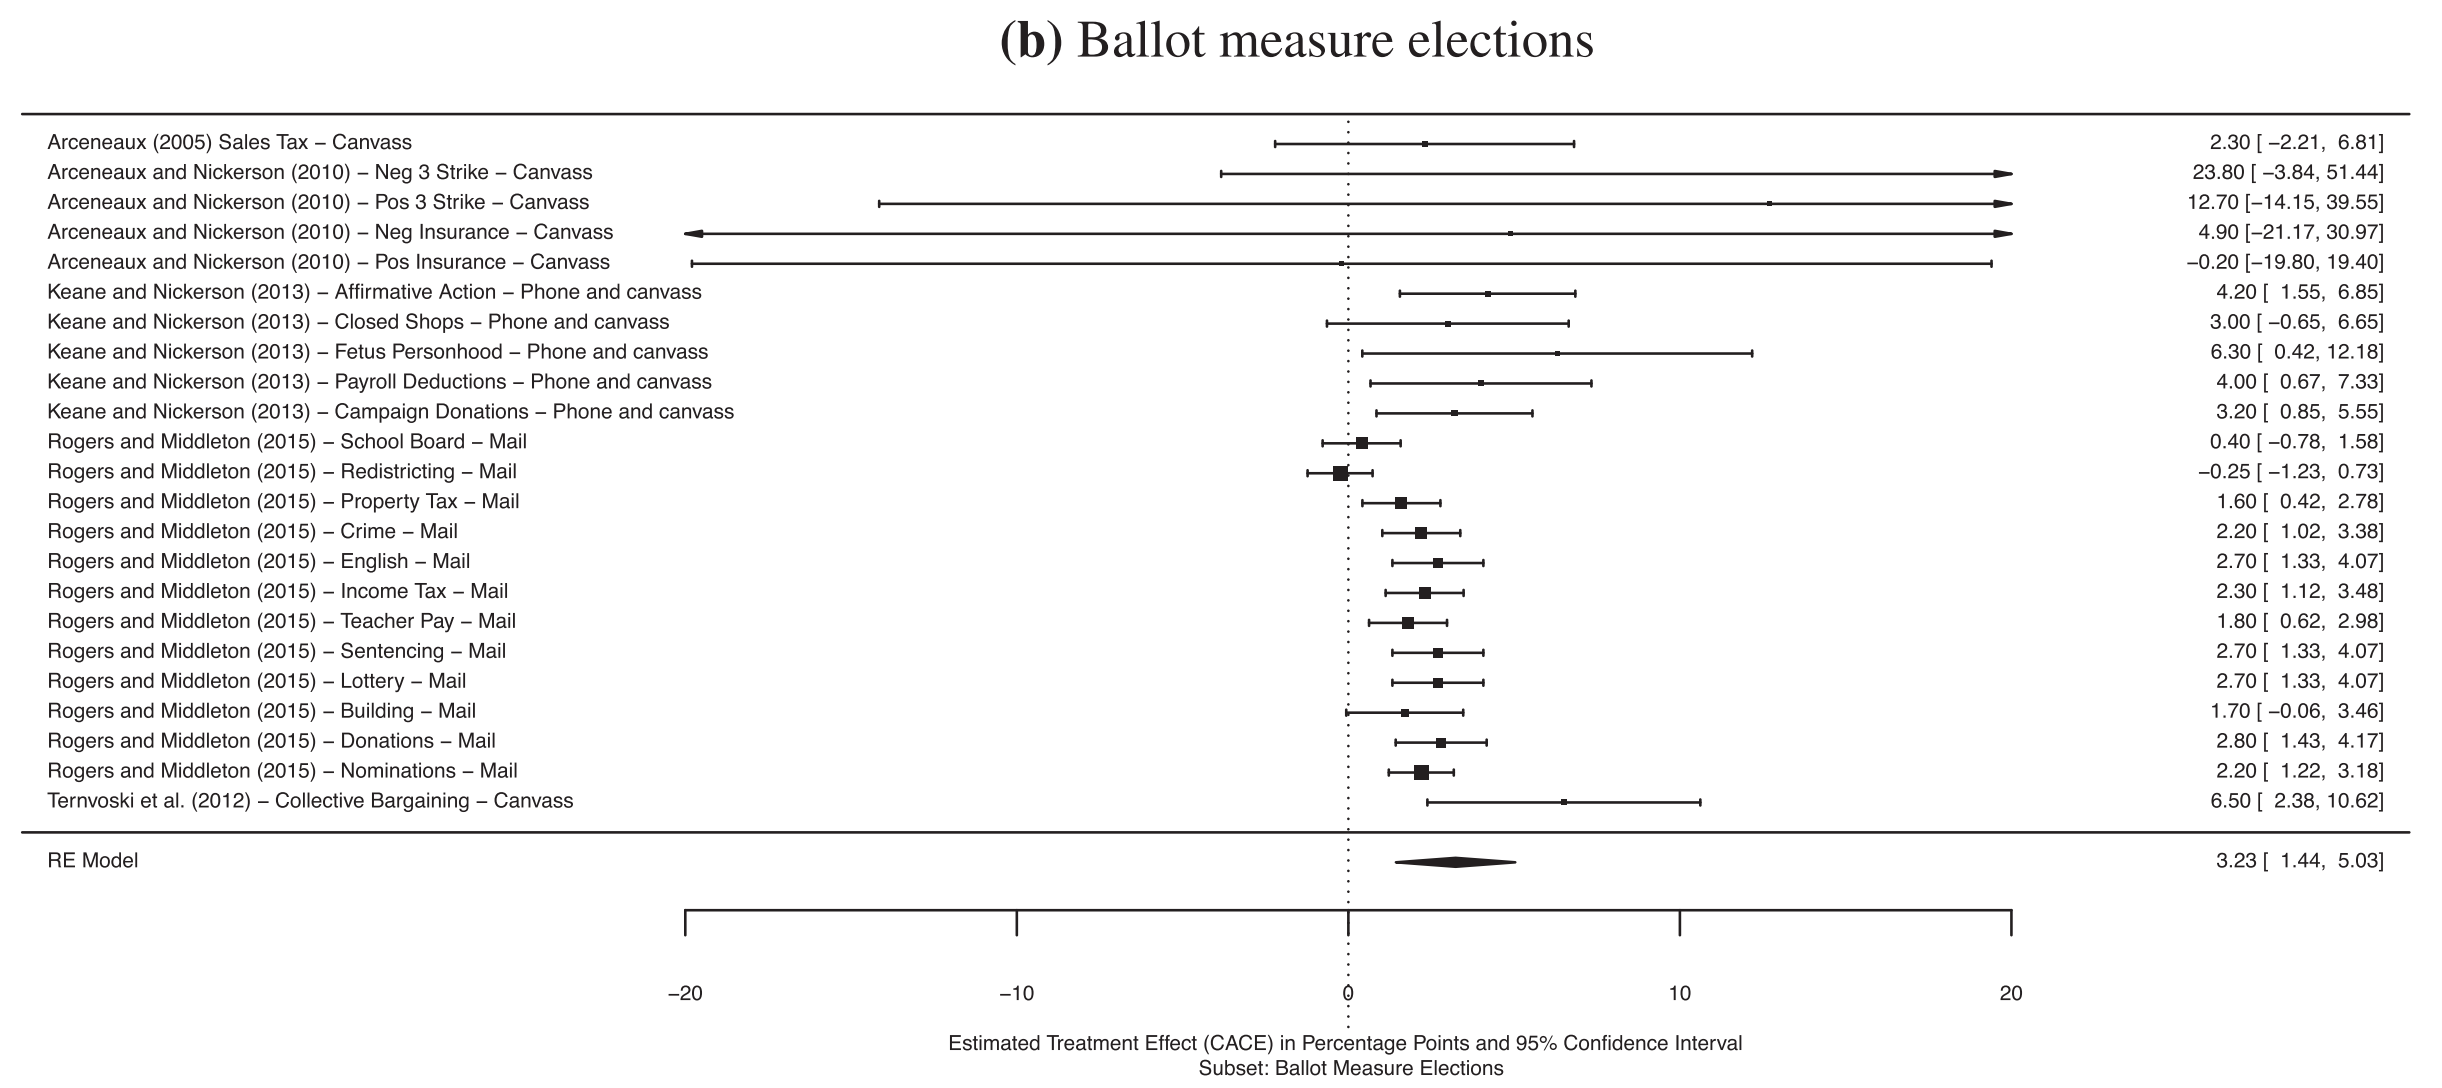
\includegraphics[scale=0.75]{meta_ballot}
\bigbreak
\caption{Meta Analysis on ballot initiatives from Kalla and Broockman 2018}
\end{figure}


\section{Experimental design: field experiment} \label{sec:Design field}

\subsection{Treatment groups and randomization} \label{sec:Treatment}

We would provide voters with different pieces of information leading to a vote on a ballot initiative. This could be different information sources (business vs advocacy group vs academic/scientific), or information vs not information. This information provision could be done through mail (a postcard) or canvassing and phone calls. Postcards: more power, and we would contribute to the literature (postcards don't work in general election campaigns - Kalla Brookman etc, but could they work on a singe, specific policy proposal). Canvassing: less power/geographic reach and probably costlier, but much higher expected treatment effect




\subsection{Outcomes} \label{sec: Outcomes}

Vote on the ballot initiative (at the precinct or smaller level).



\subsection{Choice of policy and election cycles} \label{sec:policy}

Ideal policy: a scientific consensus exists, on a technical subject on which people have very weak priors. Health care, housing, etc. 

Election cycle: off-year vs on-year election. On-year would probably give us access to a lot more voters without strong priors on the specific proposal. 


\section{Experimental design: survey experiment} \label{sec:Design survey}

\subsection{Why do a survey experiment?} \label{sec: questions}

- Methods: field vs survey experiments. Contribute to the growing evidence that survey expeiirments don't give us what we want (campaign reach outs, corruption information, etc). Do it in a very control environment: we would be able to design the syrvey so that it exactly replicates the field. 
- Our priors: survey experiments might be closer to the reality of the real world/a field experiment than in other political contexts. Because technical information, specific proposal with weak priors, no partisan shortcuts, no emotions/feelings involved bc not voting for a person. 
- If right: open the door for more survey experiments, with more ambitious treatments (fake news?). If wrong: survey experiments don't even work in a context where we felt confident that they would. Let's keep building evidence on this. 


\subsection{Design} \label{sec: questions}


\section{Potential natural experiment} \label{sec:natural}

The idea would be to use a real-life variation of information supply. Ex.: data on billboards, with their contents and where exactly they were put on, or a report sent to some precinct but not other. Info provision will probably not be random, so we would need to do a diff and diff (precinct with billboard ? precinct without billboard, but which other difference? Vote on another measure, vote in previous elections, opinion polls on the measure before billboards went up, early voting)? 

\section{Experimental analysis} \label{sec:analysis}

\subsection{Estimation of treatment effects} \label{sec:treatment_effects}

As noted above, we intend to use block random assignment in order  to increase the precision of our treatment effect estimates as well as to facilitate (preregistered) estimation of heterogenous treatment effects. Treatment effect estimates will therefore be calculated as the difference-in-means of the response rate from subjects in each of treatment groups and the response rate from subjects in the control group in each block, weighted by the number of subjects in each block relative to the total number of subjects. More formally, average treatment effects will be estimated as:

\begin{center}
$ATE = \sum_{j = 1}^{J} \frac{N_j}{N}ATE_j$
\end{center}

\noindent
where $J$ is the number of blocks, blocks are indexed by $j$, and $\frac{N_j}{N}$ represents the share of subjects who belong to block $j$. 

In practice, these differences-in-means will be calculated using a weighted least squares regression of response rate on treatment assignment, with weights corresponding to the inverse probability of treatment for each unit (IPW). All p-values will be calculated using randomization inference. As the reference/control group in the experiment is in effect the ``No information / lower tier'' treatment group, all effects must be interpreted in relation to this treatment. In other words, treatment effects should be interpreted as the change in response rate relative to the ``No information / lower tier'' group.

\subsection{Heterogenous treatment effects} \label{sec: hte}


In addition, we will test for heterogenous treatment effects on legislator party and educational attainment. Our test will take the form of regressing our outcome variable on treatments conditional upon the data representing the covariate of interest. In other words, we will split our sample by subject attributes (party and educational attainment), then estimate conditional average treatment effects (CATEs) separately for each of these attributes. For example, to test for heterogenous effects by party, we will regress outcomes on treatments for all legislators in each party. Following estimation of CATEs, we will use randomization inference to test the null hypothesis that CATEs in both groups (e.g. Democrat and Republican) equal to the ATE.

We recognize that the search for heterogenous treatment effects often suffers from the multiple comparisons problem. In a dataset with a large number of covariates, if a large enough number of subgroups is examined, it is highly likely that statistically significant interaction effects will emerge merely by chance. In other words, the more significance tests are performed, the higher the likelihood of falsely rejecting the null hypothesis at least once. We minimize this risk be preregistering our heterogenous effects of interests, as well as by performing multiple comparisons corrections using Bonferroni, Holm-Bonferroni, and Benjamin-Hochburg adjustment procedures.





\section{Conclusion} \label{sec:Conclusion}

Our next steps on this project include finalization of some of the research design decisions that remain open (i.e. federal or state level subjects, partnership with an organization, and choice of the policy). We hope to finalize these details over the summer and to preregister a final Pre-Analysis-Plan with EGAP by the end of 2019. We would then conduct the experiment in 2020. We believe that this timeline would be ideal because of the political and electoral contexts expected in 2020. An election year increases the likelihood that parties will be seeking innovative policy ideas (and decreases the time spent on other legislative activities), and it is therefore possible that legislators will be particularly responsive to information on such policies. 



\clearpage
\pagebreak
\bibliography{bibliography}

\pagebreak

\appendix
\setcounter{table}{0}
\setcounter{figure}{0}
\renewcommand\thetable{\Alph{section}.\arabic{table}}
\renewcommand\thefigure{\Alph{section}.\arabic{figure}}
\section{Appendix} \label{Appendix}





\end{document} 